% Contenidos del capítulo.
% Las secciones presentadas son orientativas y no representan
% necesariamente la organización que debe tener este capítulo.


% \subsubsection{2. Desarrollo de la Interfaz de Usuario}

% La interfaz de usuario desempeña un papel crucial en la usabilidad de la herramienta. Los objetivos relacionados con la interfaz de usuario incluyen:

% \begin{itemize}
%     \item Diseñar una interfaz de usuario intuitiva y fácil de usar para permitir a los usuarios configurar los parámetros de generación.
%     \item Implementar una interfaz de usuario que refleje de manera efectiva las opciones disponibles para la generación de terrenos.
% \end{itemize}

\section{Análisis}

\subsection{Objetivos de Implementación}

Los objetivos de implementación se centran en las metas técnicas y funcionales que se buscan alcanzar en el desarrollo de la herramienta de generación procedural de terrenos en Unity. Estos objetivos se dividen en los siguientes aspectos clave:

\subsubsection{1. Diseño de Algoritmos de Generación}

El objetivo principal en esta fase de implementación es diseñar algoritmos de generación de terrenos que sean eficientes y capaces de producir resultados convincentes. Esto incluye:

\begin{itemize}
    \item Investigar y seleccionar algoritmos de generación de terrenos adecuados para el proyecto.
    \item Diseñar algoritmos que permitan la creación de terrenos realistas y variados.
\end{itemize}

\subsubsection{2. Optimización del Rendimiento}

Para garantizar que la herramienta funcione de manera eficiente en diversas plataformas y escenarios de desarrollo, se establecen los siguientes objetivos:

\begin{itemize}
    \item Optimizar el rendimiento de los algoritmos de generación para maximizar los fotogramas por segundo.
    \item Implementar estrategias de cálculo paralelo utilizando el sistema de trabajos (Job System) de Unity para acelerar la generación de terrenos.
\end{itemize}

\subsubsection{3. Pruebas y Validación}

La validación de la herramienta es fundamental para garantizar su funcionamiento correcto. Los objetivos relacionados con las pruebas son:

\begin{itemize}
    \item Detectar posibles errores y problemas de rendimiento. Como la consistencia entre chunks vecinos dando lugar a terrenos conitnuos y la generación del terreno continua sin bajadas de fps notables.
    \item Validar que la herramienta genera terrenos realistas acorde a los parámetros con los que se configura.
    \item Comprobar que los resultados son visualmente integrables en juegos o proyectos desarrollados en Unity y que permite crear un terreno explorable.
\end{itemize}

\subsubsection{4. Mejoras en Realismo y Diferenciación de Alturas}

Además de los objetivos anteriores, se busca mejorar el realismo de los terrenos generados mediante la implementación de algoritmos de erosión. Los objetivos adicionales incluyen:

\begin{itemize}
    \item Investigar y aplicar algoritmos de erosión para simular procesos geológicos en los terrenos generados.
    \item Evaluar cómo los algoritmos de erosión mejoran la apariencia y autenticidad de los terrenos.
    \item Implementar la diferenciación de alturas en los terrenos mediante la asignación de colores según la elevación para una representación visual más rica y comprensible.
\end{itemize}

\subsection{Requisitos del Sistema}

\subsubsection{Requisitos Funcionales}

\begin{enumerate}
    \item \textbf{Generación de Terrenos:} El sistema debe ser capaz de generar terrenos de manera procedural en tiempo real, permitiendo a los usuarios especificar parámetros como tamaño, altura, erosión y demás configuraciones de terreno.
    
    \item \textbf{Continuidad del terreno:} El terreno no debe presentar discontinuidades y debe generar extensiones de terreno sin que haya una transción notable de uno a otro.
    
    \item \textbf{Algoritmos de Generación Configurables:} Los algoritmos de generación utilizados deben ser configurables, lo que permitirá a los usuarios ajustar los detalles de la generación según sus necesidades.
    
    \item \textbf{Optimización del Rendimiento:} El sistema debe estar optimizado para garantizar que la generación de terrenos sea eficiente en términos de uso de recursos y tiempos de carga.
    
    \item \textbf{Erosión Simulada:} Se deben implementar algoritmos de erosión para simular procesos geológicos y mejorar la apariencia de los terrenos generados.
    
    \item \textbf{Diferenciación de Alturas:} El sistema debe asignar colores a diferentes elevaciones del terreno para facilitar la visualización y comprensión de las características del terreno.
\end{enumerate}

\subsubsection{Requisitos No Funcionales}

\begin{enumerate}
    \item \textbf{Rendimiento:} El sistema debe ser capaz de generar terrenos en tiempo real sin experimentar retrasos notables en la ejecución.
    
    \item \textbf{Compatibilidad con Unity:} La herramienta debe integrarse perfectamente con el motor Unity, aprovechando sus capacidades y recursos.
    
    \item \textbf{Portabilidad:} El sistema debe ser compatible con múltiples plataformas y versiones de Unity, lo que permite a los desarrolladores utilizarlo en diversos proyectos.
    
    \item \textbf{Usabilidad:} El sistema debe ser intuititvo, con parámetros nombrados de manera que no cause confución en el usurio y expresen de manera clara su función.
    
    \item \textbf{Realismo Visual:} El sistema debe ser capaz de generar terrenos con realismo visual, incluyendo detalles naturales como montañas, valles.
    
    \item \textbf{Diferenciación de Alturas:} La herramienta debe permitir la diferenciación de alturas en el terreno mediante la asignación de colores o texturas específicas para representar diferentes elevaciones, facilitando la visualización y comprensión del terreno generado.

\end{enumerate}

\subsection{Arquitectura del Sistema}

\subsubsection{Visión General}
La arquitectura del sistema se basa en un enfoque modular que consta de varios componentes interconectados. El sistema se ha diseñado para ser altamente flexible y escalable, permitiendo la generación procedural de terrenos de manera eficiente. La arquitectura se centra en la generación de terrenos y su visualización en tiempo real.

\subsubsection{Componentes del Sistema}
Los componentes clave del sistema incluyen:

\begin{itemize}
    \item \textbf{Generadores del terreno:} Este componente del sistema se encargará de crear el terreno proceduralmente. Se encarga de crear la malla y de gestionar la generación de mallas en base al movimiento del usuario por el espacio. Este componente del sistema se dividirá en varias partes como veremos después en el diseño.

    \item \textbf{Generadores de altura:} Se encargan del tratamiento de las posiciones de la malla del terreno a generar, asignando alturas en base a generación de mapas de ruido en las coordeandas correspondientes al vértice.
    \item 
    \item \textbf{Generador de erosión:} Se encargará de modoifcar el mapa de alturas para producir el efecto de erosión.
    
    \item \textbf{Jobs:} Serán parte de la implementación de los generadores de terreno y altura que permitirán paralelizar sus procesos.

    \item \textbf{Generador de texturas:} Este componente se encargará la atribución de colores a los vértices para mostrar la diferencia de alturas de manera visual.    
        
    \item \textbf{Gestión de propiedades del terreno:} Componente que almacena las configuraciones del sistema, incluyendo parámetros de generación de terrenos, configuraciones de malla y opciones de visualización.
\end{itemize}

Esta arquitectura modular y bien definida permite una generación procedural de terrenos flexible y eficaz en Unity.

\subsubsection{Diagramas de Arquitectura}
A continuación, se presentan diagramas de arquitectura que muestran la estructura y las relaciones entre los componentes del sistema:

\subsubsection{Diagrama de Casos de Uso}

Para comprender mejor las interacciones entre los usuarios y el sistema, se han creado diagramas de casos de uso. Estos diagramas describen cómo los usuarios interactúan con el sistema y qué funcionalidades están disponibles para ellos.

\begin{figure}[H]
    \centering
    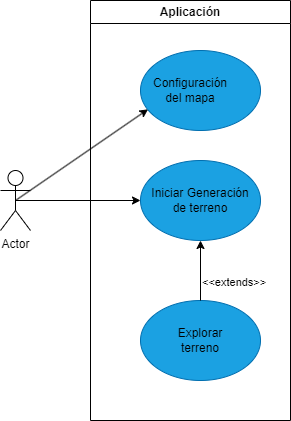
\includegraphics[width=0.5\textwidth]{img/UseCases.png}
    \caption{Diagrama de Casos de Uso del Proyecto.}
\end{figure}

\newpage
\subsubsection{Diagrama de Flujo}

El diagrama de flujo detallará, de manera general y apropiada a la fase de análisis los pasos y el flujo de las instrucciones que se llevarán a cabo para la generación infinita de terreno.

\begin{figure}[H]
    \centering
    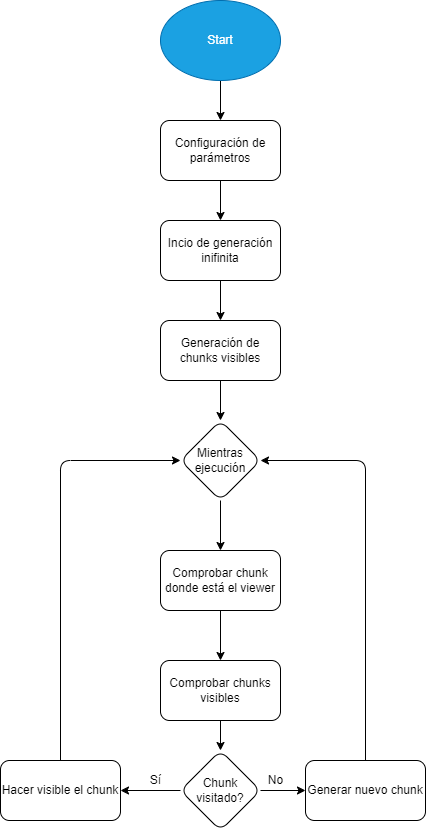
\includegraphics[width=0.6\textwidth]{img/FlowDiagramgeneracionInfinita.png}
    \caption{Diagrama de Flujo de Generación de Terreno.}
\end{figure}


\subsection{Tecnologías y Herramientas Utilizadas}

\subsubsection{Elección de Tecnologías}
La elección de las tecnologías específicas para este proyecto se basó en los siguientes criterios:

\begin{itemize}
    \item \textbf{Unity:} Se eligió Unity como motor de desarrollo debido a su versatilidad y capacidad para crear aplicaciones interactivas en 3D. Unity proporciona una amplia gama de herramientas y recursos que facilitan el desarrollo de juegos y simulaciones.
    
    \item \textbf{Unity Job System:} Para optimizar el rendimiento en la generación de terrenos, se utiliza el Unity Job System, que permite la paralelización de tareas en múltiples núcleos de CPU.
    
    \item \textbf{Burst Compiler:} La herramienta Burst Compiler se utiliza para compilar el código C \# en código nativo altamente optimizado, mejorando aún más el rendimiento de la generación de terrenos.
    
    \item \textbf{Perlin Noise, Voronoi y Simplex Noise:} Se implementan algoritmos de ruido Perli, Simplex y Voronoi para la generación de terrenos. Estos algoritmos proporcionan resultados realistas y variados.
    
\end{itemize}

Estas tecnologías se eligieron cuidadosamente para garantizar un rendimiento óptimo y una alta calidad en la generación de terrenos en tiempo real.

\subsubsection{Lenguajes de Programación}
\begin{itemize}
    \item \textbf{C\#:} Este proyecto está programado enteramente utilizando C\# como lenguaje de programación. C\# es el lenguaje que utilizan los componentes Scripts de Unity por lo que está altamente integrado con el motor, y es un lenguaje orientado a objetos que ofrece un alto rendimiento y facilidad de uso.
    
\end{itemize}

\subsubsection{Herramientas de Desarrollo}

Durante el desarrollo de este proyecto, se utilizaron diversas herramientas y software que desempeñaron un papel fundamental en la planificación, implementación y gestión del trabajo. A continuación, se detallan las principales herramientas de desarrollo utilizadas:

\begin{itemize}
    \item \textbf{IDE Principal:} JetBrains Rider fue el IDE principal utilizado para el desarrollo en C\#. Rider proporcionó un entorno de desarrollo integrado eficiente y potente para la escritura de código, depuración y pruebas del proyecto.
    
    \item \textbf{Visual Studio:} Visual Studio se utilizó específicamente para la creación de diagramas de clases, lo que permitió una representación visual clara de la estructura del proyecto y las relaciones entre las clases.
    
    \item \textbf{VS Code:} Visual Studio Code, junto con el plugin draw.io, se utilizó para crear varios tipos de diagramas, incluidos los diagramas de casos de uso y diagramas de flujo. Estas representaciones gráficas ayudaron a comprender y comunicar el flujo de trabajo del sistema. También se suó para la redacción en Latex de la memoria.
        
    \item \textbf{Control de Versiones (Git y GitHub):} Git se utilizó para el control de versiones del código fuente del proyecto. GitHub se empleó como plataforma de alojamiento para el repositorio de Git, lo que facilitó la colaboración en equipo y el seguimiento de cambios.
    
    \item \textbf{Gestión de Tareas (Trello):} Trello se utilizó para la gestión de tareas y la planificación del proyecto. La herramienta permitió organizar y priorizar tareas, así como realizar un seguimiento del progreso de cada elemento del proyecto.
    
    \item \textbf{Burst Compiler:} El Burst Compiler se utilizó para compilar el código C\# en código nativo altamente optimizado, lo que contribuyó significativamente a mejorar el rendimiento en la generación de terrenos.
\end{itemize}

Estas herramientas desempeñaron un papel esencial en la realización exitosa del proyecto, proporcionando las capacidades necesarias para el desarrollo, la documentación, la colaboración en equipo y la optimización de rendimiento.

\subsubsection{Alternativas Consideradas}
Antes de tomar las decisiones de diseño finales, se consideraron varias alternativas, incluyendo:

\begin{itemize}
    \item \textbf{Otras Tecnologías de Generación de Terrenos:} Se evaluaron diferentes tecnologías y enfoques para la generación de terrenos, como el uso de mapas de altura pregenerados versus generación procedural en tiempo real.
    
    \item \textbf{Métodos de Optimización:} Se exploraron diversas técnicas de optimización además del Unity Job System, como el uso de GPU para cálculos intensivos o la paralelización mediante threads manual.
    
    \item \textbf{Otros Algoritmos de Ruido:} Se investigaron algoritmos de ruido alternativos además de Perlin y Simplex para determinar cuáles producirían los resultados deseados y técnicas de generación, como el algoritmo diamante-cuadrado. Pero se optó por el ruido debido a que facilitaba la consistencia entre lso bordes de partes de terreno nuevas generadas
\end{itemize}

\subsection{Planificación del Desarrollo}

\subsubsection{Metodología de Desarrollo}
El proyecto siguió una metodología de desarrollo ágil, lo que permitió una adaptación flexible a medida que se abordaban nuevas fases del desarrollo y se tomaban nuevas decisiones de implementación o diseño. Se realizaron reuniones periódicas de revisión y planificación para ajustar el enfoque según fuera necesario. Cada día se fueron subiendo incrementos de desarrollo al repositorio remoto, gestioando un control de cuáles habían sido las mejroas subidas, cuál era el estado del proyecto y cuáles debían ser los siguientes objetivos.

\subsubsection{Gestión de Tiempo}
La gestión del tiempo se realizó mediante una planificación detallada en Trello. Creando pilas de tareas "por hacer", "en desarrollo", "termiandas" y "mejorables".

La planificación del proyecto se ha desglosado en las siguientes fases, las cuales culminan con sus correspondientes hitos.
\begin{itemize}
    \item Análisis preeliminar: Esta fase es en la que se determinan los objetivos, los requisitos, alcance del proyecto y se hace una investigación sobre los recursos que se pueden emplear para el proyecto. Esta fase culmina con el hito de la aprobación del análsis preeliminar.
    \item Fase de Análisis: Esta fase corresponde como su propio nombre indica al análisis del proyecto: estudio de requisitos, de la arquitectura que se va a diseñar y de los procesos y componentes necesarios para el proyecto. esta fase culmina.Esta fase culmina con el hito de la aprobación del análsis.
    \item Fase de Diseño: En la fase de diseño se diseñará la estructura de la arquitectura que tendrá la herramienta, los componentes y relaciones entre ellos, así como los parámetros que tendrá de el ususrio para configurar la generación de terreno. Esta fase culmina con la aprobcación del diseño.
    \item Implementación: Durante la implementación se implementan todos los compoentnes, clases y procesos necesarios. Culmina con el finde la implementación y comienzo de las pruebas.
    \item Pruebas y resutlados: Aquí se desarrollan diferentes pruebasy correcciones sobre la implementación anterior. Esta fase culmina con la aprobación de los resutladso de las últimas pruebas que se realicen.
    \item Finalización de la documentación: El hito de la finalización de la documentación culmina con la entrega de la memoria y el video explicativo de este proyecto.
\end{itemize}

El cronograma de desarrollo detallado se encuentra en el apéndice A para una referencia más completa.

\subsubsection{Recursos Necesarios}
Los recursos necesarios para llevar a cabo el desarrollo incluyeron:

\begin{itemize}
    \item Personal de Desarrollo: Para este proyecto el personal fue una única persona que ocupó todos los roles del desarrollo y un product owner que especificaba los requisitos que debía cumplir el proyecto.
    
    \item Hardware: Se utilizó un equipo portátil con procesador i5-11400H con 2.7GHz, 16 GB de RAM, 1TB de memoria en disco y tarjeta gráfica NVidia 3060 con 6GB de RAM. El equipo contaba con windows 10 Home como sistema operativo. 
    
    \item Software: Se requirieron herramientas como Unity, JetBrains Rider, Visual Studio, VS Code con el plugin draw.io, LaTeX y el Burst Compiler para el desarrollo y la documentación del proyecto.
\end{itemize}

